\chapter{Definition of Hilbert Complexes}\label{sec:Hilbert complex definitions}
    Define the following Hilbert spaces and exact complexes:
    
    \section*{1D in Time}
         On $[0, T]$:
        
        \subsection*{$H\Lambda^{\bullet}([0, T])$}
            Define the Hilbert spaces: \BA{(I haven't really defined what norms these spaces use... Not sure I need to really though...)}
            \begin{align}
                L^{2}  :=  \left\{u \in L^{1}_{\rm loc} : \|u\|_{[0, T]} < \infty\right\},  &&
                H^{1}  :=  \left\{u \in L^{1}_{\rm loc} : \partial_{t}u \in L^{2}\right\}
            \end{align}
            Define the exact complex $H\Lambda^{\bullet}([0, T])$:
            \begin{center}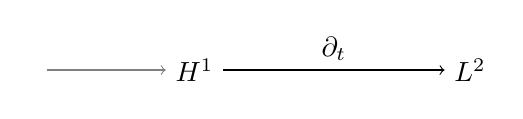
\begin{tikzpicture}[align = center, node distance = 4cm, auto]
                \node (R)  at (- 2, 0) {\color{black!50} $\bbR$};
                \node (H1) at (0,   0) {$H^{1}$};
                \node (L2) at (3.5, 0) {$L^{2}$};
    
                \draw[->, draw = black!50] (R)  -- (H1);
                \draw[->] (H1) -- (L2) node[above, midway] {$\partial_{t}$};
            \end{tikzpicture}\end{center}

        \subsection*{$H_{0}\Lambda^{\bullet}([0, T])$}
            Define the Hilbert space:
            \begin{equation}
                H^{1}_{0}  :=  \left\{u \in H^{1} : u = 0|_{t \in \{0, T\}}\right\}
            \end{equation}
            Define the exact complex $H_{0}\Lambda^{\bullet}([0, T])$:
            \begin{center}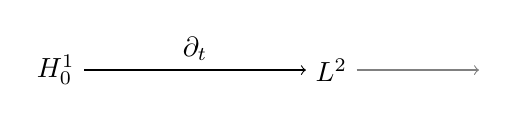
\begin{tikzpicture}[align = center, node distance = 4cm, auto]
                \node (H1) at (0,   0) {$H^{1}_{0}$};
                \node (L2) at (3.5, 0) {$L^{2}$};
                \node (R)  at (5.5, 0) {\color{black!50} $\bbR$};
    
                \draw[->] (H1) -- (L2) node[above, midway] {$\partial_{t}$};
                \draw[->, draw = black!50] (L2) -- (R);
            \end{tikzpicture}\end{center}

        \subsection*{$H_{\pm}\Lambda^{\bullet}([0, T])$}
            Define the Hilbert spaces:
            \begin{align}
                H^{1}_{+}  &:=  \left\{u \in H^{1} : u = 0|_{t = T}\right\}  \\
                H^{1}_{-}  &:=  \left\{u \in H^{1} : u = 0|_{t = 0}\right\}
            \end{align}
            Define the exact complexes $H_{\pm}\Lambda^{\bullet}(\bfOmega)$:
            \begin{center}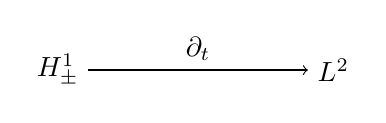
\begin{tikzpicture}[align = center, node distance = 4cm, auto]
                \node (H1) at (0,   0) {$H^{1}_{\pm}$};
                \node (L2) at (3.5, 0) {$L^{2}$};
    
                \draw[->] (H1) -- (L2) node[above, midway] {$\partial_{t}$};
            \end{tikzpicture}\end{center}
            
            \BA{TO ADD:
            \begin{itemize}
                \item  Proofs of energy/helicity/Gauss's law conservation (Modify weak formulations accordingly)
                \item  Commutative diagram/references for tensor product complexes
                \item  Notes about what conformity I need for my function spaces/how to handle the weak formulation for non-conforming discretizations
    `               \item  Continuity of helicity
            \end{itemize}}
        
    \section*{3D in Space}
        On $\bfOmega$:

        \subsection*{$H\Lambda^{\bullet}(\bfOmega)$}
            Define the Hilbert spaces: \BA{(Bit of a clash in notation here on the $L^{2}$'s.)}
            \begin{align}
                L^{2}          &:=  \left\{u \in L^{1}_{\rm loc} : \|u\|_{\bfOmega} < \infty\right\}  \\
                \bfH(\rmdiv)   &:=  \left\{\bfu \in \left(L^{1}_{\rm loc}\right)^{3} : \nabla\cdot\bfu \in L^{2}\right\}  \\
                \bfH(\bfcurl)  &:=  \left\{\bfu \in \left(L^{1}_{\rm loc}\right)^{3} : \nabla\wedge\bfu \in \left(L^{2}\right)^{3}\right\}  \\
                H^{1}          &:=  \left\{u \in L^{1}_{\rm loc} : \nabla u \in \left(L^{2}\right)^{3}\right\}
            \end{align}
            Define the exact complex of vector proxies for $H\Lambda^{\bullet}(\bfOmega)$: \BA{([Ref])}
            \begin{center}\begin{tikzpicture}[align = center, node distance = 4cm, auto]
                \node (R)     at (- 2,  0) {\color{black!50} $\bbR$};
                \node (H1)    at (0,    0) {$H^{1}$};
                \node (Hcurl) at (3.5,  0) {$\bfH(\bfcurl)$};
                \node (Hdiv)  at (7,    0) {$\bfH(\rmdiv)$};
                \node (L2)    at (10.5, 0) {$L^{2}$};
    
                \draw[->, draw = black!50] (R) -- (H1);
                \draw[->] (H1)    -- (Hcurl) node[above, midway] {$\bfgrad$};
                \draw[->] (Hcurl) -- (Hdiv)  node[above, midway] {$\bfcurl$};
                \draw[->] (Hdiv)  -- (L2)    node[above, midway] {$\rmdiv$};
            \end{tikzpicture}\end{center}

        \subsection*{$H_{0}\Lambda^{\bullet}(\bfOmega)$}
            Define the Hilbert spaces:
            \begin{align}
                \bfH_{0}(\rmdiv)   &:=  \left\{\bfu \in \bfH(\rmdiv) : \bfu\cdot\bfn = 0|_{\bfGamma}\right\}  \\
                \bfH_{0}(\bfcurl)  &:=  \left\{\bfu \in \bfH(\bfcurl) : \bfu\wedge\bfn = \bfzero|_{\bfGamma}\right\}  \\
                H^{1}_{0}          &:=  \left\{u \in H^{1} : u = 0|_{\bfGamma}\right\}
            \end{align}
            Define the exact complex of vector proxies for $H_{0}\Lambda^{\bullet}(\bfOmega)$: \BA{([Ref])}
            \begin{center}\begin{tikzpicture}[align = center, node distance = 4cm, auto]
                \node (H1)    at (0,    0) {$H^{1}_{0}$};
                \node (Hcurl) at (3.5,  0) {$\bfH_{0}(\bfcurl)$};
                \node (Hdiv)  at (7,    0) {$\bfH_{0}(\rmdiv)$};
                \node (L2)    at (10.5, 0) {$L^{2}$};
                \node (R)     at (12.5, 0) {\color{black!50} $\bbR$};
    
                \draw[->] (H1)    -- (Hcurl) node[above, midway] {$\bfgrad$};
                \draw[->] (Hcurl) -- (Hdiv)  node[above, midway] {$\bfcurl$};
                \draw[->] (Hdiv)  -- (L2)    node[above, midway] {$\rmdiv$};
                \draw[->, draw = black!50] (L2) -- (R);
            \end{tikzpicture}\end{center}
            
        \subsection*{$H_{0}\Lambda^{\bullet}(\bfOmega)$}
            For $\emptyset  \subset  \bfgamma  \subset  \bfGamma$, define the Hilbert spaces:
            \begin{align}
                \bfH_{\bfgamma}(\rmdiv)   &:=  \left\{\bfu \in \bfH(\rmdiv) : \bfu\cdot\bfn = 0|_{\bfgamma}\right\}  \\
                \bfH_{\bfgamma}(\bfcurl)  &:=  \left\{\bfu \in \bfH(\bfcurl) : \bfu\wedge\bfn = \bfzero|_{\bfgamma}\right\}  \\
                H^{1}_{\bfgamma}          &:=  \left\{u \in H^{1} : u = 0|_{\bfgamma}\right\}
            \end{align}
            Define the exact complex of vector proxies for $H_{0}\Lambda^{\bullet}(\bfOmega)$: \BA{([Ref])}
            \begin{center}\begin{tikzpicture}[align = center, node distance = 4cm, auto]
                \node (H1)    at (0,    0) {$H^{1}_{\bfgamma}$};
                \node (Hcurl) at (3.5,  0) {$\bfH_{\bfgamma}(\bfcurl)$};
                \node (Hdiv)  at (7,    0) {$\bfH_{\bfgamma}(\rmdiv)$};
                \node (L2)    at (10.5, 0) {$L^{2}$};
                
                \draw[->] (H1)    -- (Hcurl) node[above, midway] {$\bfgrad$};
                \draw[->] (Hcurl) -- (Hdiv)  node[above, midway] {$\bfcurl$};
                \draw[->] (Hdiv)  -- (L2)    node[above, midway] {$\rmdiv$};
            \end{tikzpicture}\end{center}
        
    \section*{(3+1)D in Space and Time}
        \BA{Talk about tensor product subcomplexes.}
        
        On $\bfOmega\otimes[0, T]$:

        \subsection*{$H\Lambda^{\bullet}(\bfOmega\otimes[0, T])$}
            Define the Hilbert spaces:
            \begin{align}
                L^{2}  &:=  \left\{u \in L^{1}_{\rm loc} : \|u\|_{\bfOmega\otimes[0, T]} < \infty\right\}  \\
                \bfH(\partial_{t} + \rmdiv)  &:=  \left\{\begin{pmatrix} u \\ \bfv \end{pmatrix} \in \left(L^{1}_{\rm loc}\right)^{1 + 3} : \partial_{t}u + \nabla\cdot\bfv \in L^{2}\right\}  \\
                \bfH\left(\begin{matrix} * - \rmdiv \\ \bfcurl + \partial_{t} \end{matrix}\right)  &:=  \left\{\begin{pmatrix} \bfu \\ \bfv \end{pmatrix} \in \left(L^{1}_{\rm loc}\right)^{3 + 3} : \begin{pmatrix} - \nabla\cdot\bfv \\ \nabla\wedge\bfu + \partial_{t}\bfv \end{pmatrix} \in \left(L^{2}\right)^{1 + 3}\right\}  \\
                \bfH\left(\begin{matrix} \bfgrad + \partial_{t} \\ * - \bfcurl \end{matrix}\right)  &:=  \left\{\begin{pmatrix} u \\ \bfv \end{pmatrix} \in \left(L^{1}_{\rm loc}\right)^{1 + 3} : \begin{pmatrix} \nabla u + \partial_{t}\bfv \\ - \nabla\wedge\bfv \end{pmatrix} \in \left(L^{2}\right)^{3 + 3}\right\}  \\
                H^{1}  &:=  \left\{u \in L^{1}_{\rm loc} : \begin{pmatrix} \partial_{t}u \\ - \nabla u \end{pmatrix} \in \left(L^{2}\right)^{1 + 3}\right\}
            \end{align}
            Define the exact complex of vector proxies for $H\Lambda^{\bullet}(\bfOmega)$: \BA{([Ref])}
            {\scriptsize \begin{center}\begin{tikzpicture}[align = center, node distance = 4cm, auto]
                \node (R)   at (- 1.5, 0) {\color{black!50} $\bbR$};
                \node (HL0) at (0,     0) {$H^{1}$};
                \node (HL1) at (3,     0) {$\bfH\left(\begin{matrix} \bfgrad + \partial_{t} \\ * - \bfcurl \end{matrix}\right)$};
                \node (HL2) at (7.5,   0) {$\bfH\left(\begin{matrix} * - \rmdiv \\ \bfcurl + \partial_{t} \end{matrix}\right)$};
                \node (HL3) at (11.5,  0) {$\bfH(\partial_{t} + \rmdiv)$};
                \node (HL4) at (14,    0) {$L^{2}$};

                \draw[->, black!50] (R) -- (HL0);
                \draw[->] (HL0) -- (HL1) node[above, midway] {$\left(\begin{matrix} \partial_{t} \\ - \bfgrad \end{matrix}\right)$};
                \draw[->] (HL1) -- (HL2) node[above, midway] {$\left(\begin{matrix} \bfgrad + \partial_{t} \\ * - \bfcurl \end{matrix}\right)$};
                \draw[->] (HL2) -- (HL3) node[above, midway] {$\left(\begin{matrix} * - \rmdiv \\ \bfcurl + \partial_{t} \end{matrix}\right)$};
                \draw[->] (HL3) -- (HL4) node[above, midway] {$\partial_{t} + \rmdiv$};
            \end{tikzpicture}\end{center}}

        \subsection*{$H_{0}\Lambda^{\bullet}(\bfOmega\otimes[0, T])$}
            Define the Hilbert spaces: \BA{(Think some of the BCs might be slightly wrong here...)}
            \begin{align}
                L^{2}_{0}  &:=  \left\{u \in L^{2} : \int_{\bfOmega\otimes[0, T]}u = 0\right\}  \\
                \bfH_{0}(\partial_{t} + \rmdiv)  &:=  \left\{\begin{pmatrix} u \\ \bfv \end{pmatrix} \in \bfH(\partial_{t} + \rmdiv) : \bfv\cdot\bfn|_{\bfGamma\otimes[0, T]}, u|_{\bfOmega\otimes\{0, T\}} = 0\right\}  \\
                \bfH_{0}\left(\begin{matrix} * - \rmdiv \\ \bfcurl + \partial_{t} \end{matrix}\right)  &:=  \left\{\begin{pmatrix} \bfu \\ \bfv \end{pmatrix} \in \bfH\left(\begin{matrix} * - \rmdiv \\ \bfcurl + \partial_{t} \end{matrix}\right) : \begin{matrix} \bfv\cdot\bfn|_{\bfGamma\otimes[0, T]} = 0 \\ \bfu\wedge\bfn|_{\bfOmega\otimes\{0, T\}}, \bfv|_{\bfGamma\otimes[0, T]} = \bfzero \end{matrix}\right\}  \\
                \bfH_{0}\left(\begin{matrix} \bfgrad + \partial_{t} \\ * - \bfcurl \end{matrix}\right)  &:=  \left\{\begin{pmatrix} u \\ \bfv \end{pmatrix} \in \bfH\left(\begin{matrix} \bfgrad + \partial_{t} \\ * - \bfcurl \end{matrix}\right) : \begin{matrix} u\bfn|_{\bfGamma\otimes[0, T]}, \bfv|_{\bfOmega\otimes\{0, T\}} = \bfzero \\ \bfv\wedge\bfn|_{\bfGamma\otimes[0, T]} = \bfzero \end{matrix}\right\}  \\
                H^{1}_{0}  &:=  \left\{u \in H^{1} : \begin{matrix} u = 0|_{\bfOmega\otimes\{0, T\}} \\ u = 0|_{\bfGamma\otimes[0, T]} \end{matrix}\right\}
            \end{align}
            Define the exact complex of vector proxies for $H_{0}\Lambda^{\bullet}(\bfOmega)$: \BA{([Ref])}
            {\scriptsize \begin{center}\begin{tikzpicture}[align = center, node distance = 4cm, auto]
                \node (HL0) at (0,    0) {$H^{1}_{0}$};
                \node (HL1) at (3,    0) {$\bfH_{0}\left(\begin{matrix} \bfgrad + \partial_{t} \\ * - \bfcurl \end{matrix}\right)$};
                \node (HL2) at (7.5,  0) {$\bfH_{0}\left(\begin{matrix} * - \rmdiv \\ \bfcurl + \partial_{t} \end{matrix}\right)$};
                \node (HL3) at (11.5, 0) {$\bfH_{0}(\partial_{t} + \rmdiv)$};
                \node (HL4) at (14,   0) {$L^{2}_{0}$};
    
                \draw[->] (HL0) -- (HL1) node[above, midway] {$\left(\begin{matrix} \partial_{t} \\ - \bfgrad \end{matrix}\right)$};
                \draw[->] (HL1) -- (HL2) node[above, midway] {$\left(\begin{matrix} \bfgrad + \partial_{t} \\ * - \bfcurl \end{matrix}\right)$};
                \draw[->] (HL2) -- (HL3) node[above, midway] {$\left(\begin{matrix} * - \rmdiv \\ \bfcurl + \partial_{t} \end{matrix}\right)$};
                \draw[->] (HL3) -- (HL4) node[above, midway] {$\partial_{t} + \rmdiv$};
            \end{tikzpicture}\end{center}}

        \subsection*{$H_{\pm}\Lambda^{\bullet}(\bfOmega\otimes[0, T])$}
            For $\tau_{\pm}$ defined $\tau_{+}  :=  T$, $\tau_{-}  :=  0$, define the Hilbert spaces:
            \begin{align}
                \bfH_{\pm}(\partial_{t} + \rmdiv)  &:=  \left\{\begin{pmatrix} u \\ \bfv \end{pmatrix} \in \bfH(\partial_{t} + \rmdiv) : \bfv\cdot\bfn|_{\bfGamma\otimes[0, T]}, u|_{\bfOmega\otimes\{\tau_{\pm}\}} = 0\right\}  \\
                \bfH_{\pm}\left(\begin{matrix} * - \rmdiv \\ \bfcurl + \partial_{t} \end{matrix}\right)  &:=  \left\{\begin{pmatrix} \bfu \\ \bfv \end{pmatrix} \in \bfH\left(\begin{matrix} * - \rmdiv \\ \bfcurl + \partial_{t} \end{matrix}\right) : \begin{matrix} \bfv\cdot\bfn|_{\bfGamma\otimes[0, T]} = 0 \\ \bfu\wedge\bfn|_{\bfOmega\otimes\{\tau_{\pm}\}}, \bfv|_{\bfGamma\otimes[0, T]} = \bfzero \end{matrix}\right\}  \\
                \bfH_{\pm}\left(\begin{matrix} \bfgrad + \partial_{t} \\ * - \bfcurl \end{matrix}\right)  &:=  \left\{\begin{pmatrix} u \\ \bfv \end{pmatrix} \in \bfH\left(\begin{matrix} \bfgrad + \partial_{t} \\ * - \bfcurl \end{matrix}\right) : \begin{matrix} u\bfn|_{\bfGamma\otimes[0, T]}, \bfv|_{\bfOmega\otimes\{\tau_{\pm}\}} = \bfzero \\ \bfv\wedge\bfn|_{\bfGamma\otimes[0, T]} = \bfzero \end{matrix}\right\}  \\
                H^{1}_{\pm}  &:=  \left\{u \in H^{1} : \begin{matrix} u = 0|_{\bfOmega\otimes\{\tau_{\pm}\}} \\ u = 0|_{\bfGamma\otimes[0, T]} \end{matrix}\right\}
            \end{align}
            Define the exact complex of vector proxies for $H_{\pm}\Lambda^{\bullet}(\bfOmega)$: \BA{([Ref])}
            {\scriptsize \begin{center}\begin{tikzpicture}[align = center, node distance = 4cm, auto]
                \node (HL0) at (0,    0) {$H^{1}_{\pm}$};
                \node (HL1) at (3,    0) {$\bfH_{\pm}\left(\begin{matrix} \bfgrad + \partial_{t} \\ * - \bfcurl \end{matrix}\right)$};
                \node (HL2) at (7.5,  0) {$\bfH_{\pm}\left(\begin{matrix} * - \rmdiv \\ \bfcurl + \partial_{t} \end{matrix}\right)$};
                \node (HL3) at (11.5, 0) {$\bfH_{\pm}(\partial_{t} + \rmdiv)$};
                \node (HL4) at (14,   0) {$L^{2}$};
    
                \draw[->] (HL0) -- (HL1) node[above, midway] {$\left(\begin{matrix} \partial_{t} \\ - \bfgrad \end{matrix}\right)$};
                \draw[->] (HL1) -- (HL2) node[above, midway] {$\left(\begin{matrix} \bfgrad + \partial_{t} \\ * - \bfcurl \end{matrix}\right)$};
                \draw[->] (HL2) -- (HL3) node[above, midway] {$\left(\begin{matrix} * - \rmdiv \\ \bfcurl + \partial_{t} \end{matrix}\right)$};
                \draw[->] (HL3) -- (HL4) node[above, midway] {$\partial_{t} + \rmdiv$};
            \end{tikzpicture}\end{center}}
    